\pagenumbering{arabic}
\chapter{Introduction}
\minitoc



\section{Motivation}
Computers have become an important part of our lives. They have moved from being just equipment for managing business and office tasks to being a real partner in social communication and interaction with humans. The prevalence in the past two decades of small computers such as laptops, mobile phones and tablet devices has played a significant role in making the computers a permanent companion of our lives and our relationships with others. 

Our emotions critically affect all aspects of our lives, from how we live, work, learn and play, to our decisions, big and small. Facial expression has a significant role in our communication with others. 
Today, mobile phones and computers are a significant way to communicate with others, so machines have to perform lots of human tasks, and need to have more human-like capabilities.
Human emotional intelligence depends on our ability to recognise not only our own emotions but also those of other people; to this end, smart devices and advanced AI (artificial intelligence) systems should have the capacity to understand our emotions and interact with humans emotionally. Human-computer intelligent interaction (HCII) is a growing field that aims to achieve that.  
Human faces are the most important part of the human body to express feelings. People around the world use similar facial expressions to express emotions, such as happiness, sadness, anger, disgust, surprise and fear. Facial expressions enable people to understand each other; sometimes without even one single word, or in other words, facial expressions are a global language.

Most proposed automatic facial-expression recognition methods have been based on unnatural facial expressions, using databases that have been built from acted facial expressions. The creators of those databases have asked models or actors to express some facial expressions, and the problem here that the real emotions are different than those posed.

Nowadays, facial emotional recognition systems  have been used in several applications \citep{khan2013detection} such as:
\begin{enumerate}
	\item Detection and treatment of of depression and anxiety \citep{ekman1997face}.
	\item EmotiChat \citep{anderson2006real} .
	\item Smart homes \citep{pantic2007human}.
	\item Affective/social robots \citep{scherer2010blueprint}.
	\item Emotientv \citep{Whitehill2014AutomaticFE}.
	\item EmoVu 
	
\end{enumerate}




\section{Facial expression recognition systems}
%%%%%%%%%%%%%%%%%%%%%%%%%%%%%%%%%%%%%%%%%%%%%%%%%%%%%%%%%%%%%%%%%
\begin{figure}[t]
	\centering
	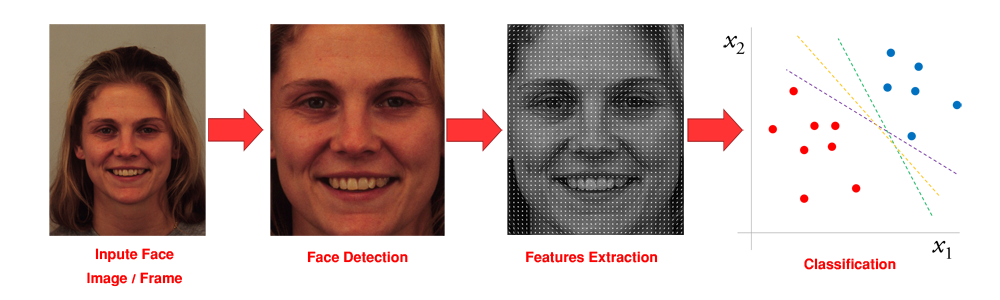
\includegraphics[width=1\textwidth]{Chapter1/Figs/MainSystem.png}
	\textbf{
		\caption{Basic facial expression recognition system pipeline}
		\label{fig:MainSystem}}
\end{figure}
%%%%%%%%%%%%%%%%%%%%%%%%%%%%%%%%%%%%%%%%%%%%%%%%%%%%%%%%%%%%%%%%%

Facial expression recognition systems follow the same general steps as illustrated in figure \ref{fig:MainSystem}.
The first is to find the Region Of Interest (ROI), which is the face. Unwanted areas may badly affect classification accuracy. Many facial detection methods have been proposed, such as the Viola-Jones algorithm \citep{viola2004robust,viola2001rapid}. 

The next step is extracting the features from a detected face. The purpose of image feature extraction is to describe an image efficiently by extracting the essential values and reduce the data without losing any significant details.  There are many ways to do that, some depending on image texture itself, while other methods describe the image geometrically.

The last step is to classify the extracted features. In this step, machine learning plays the primary role in finding the differences between feature groups and making a decision as to what a group of values refers. 

Some facial expression reconnection methods may contain further steps to improve accuracy: for example, applying some pre-process techniques to enhance the image before feature extraction, or reducing the length of the extracted features vector.  



%\section{Applications}

\section{Challenges}
Although many methods have been proposed for facial expression recognition, many challenges and difficulties are still facing this field, especially with natural expressions.

\begin{enumerate}
	\item The very similarity of facial expressions means that many people find it difficult to identify the differences between certain expressions, for example, fear and surprise. We did a study,  asking people to identify a range of facial expressions, and we found a significant variation in people's ability to determine facial expressions particularly these representing emotions such as anger and fear.
	
	\item There is variation amongst human faces and their ways to express their emotions. Some people exaggerate their expressions, while others try to hide them. Moreover, there are many primary facial expressions and some secondary expressions, and this may change according to cultures and nations.
	
	\item Most of the facial expression datasets contain unnatural facial expressions and have been built depending on acted facial expressions by some models or actors. These expressions are not indicative of the way people do in real life.
	
	\item We have found that all the studied facial expression recognition methods are computationally expensive because they usually require large feature vector dimensionally. This makes difficulty for real-time applications and hinders the achievement of good results on different datasets.
\end{enumerate}



\section{Contributions}
\begin{itemize}
	\item We used the Labelled Faces in the wild dataset to provide a new facial expression dataset (eLWF) by involving people in the labelling process. The new dataset contains natural facial expressions rather than most of the current datasets which depend on actors mimicking facial expressions.     
	\item We show that a combination of three image feature extraction methods Locally Binary Patterns(LBP) \citet{ojala1996comparative}, Histogram of oriented gradients (HOG) \citep{dalal2005histograms}, and Dense speeded up robust features (D-SURF)  \citep{bay2006surf,bay2008speeded} gives better image description than using only one of them and that this improves the classification rate with SVM and Random forests.  
	\item We propose a new method to identify the most relevant image regions for emotion classification.
	
	\item We describe a new weighted voting algorithm, in which the weighted predictions of classifiers trained on pairs of classes are combined with the weights learned using an evolutionary algorithm.  This method yields superior results, particularly for the hard-to-distinguish emotions.
	
	\item We used smoothing techniques to reduce the video classification errors (noise), by relying on a set of sequential video frames. We have employed a video database called DynEmo \citep{tcherkassof2013dynemo} developed by psychologists in our experiments, which contains videos of real facial emotions, and we labelled the videos based on frames rather than time. 
\end{itemize}




\section{Publications}

\textbf{The materials presented in chapters 3 and 4 have been published in:}

Abuhammad, H., \& Everson, R. (2018, June). Emotional Faces in the Wild: Feature Descriptors for Emotion Classification. In International Conference Image Analysis and Recognition (pp. 164-174). Springer, Cham. 



\citep{abuhammad2018emotional}


\section{Structure of the thesis}
The rest of the thesis is structured as follows.

\textbf{Chapter 2} 
\textcolor{red}{
	We present a brief overview of some related features extraction methods, together with Random forest and support vector machine classifiers. Moreover, we present a brief overview of three optimisation methods: Nelder-Mead simplex direct search, Bayesian optimisation and the Covariance Matrix Adaptation Evolution Strategy. 
	In particular, we discuss related methods of facial expression methods which depend on image-appearance techniques.}

\textbf{Chapter 3}

In this chapter,  we introduce the new ``Emotional Faces in the Wild'' dataset (eLFW) \citep{LFWTech,LFWTechUpdate},  a citizen-labelling of 1310 faces from the Labelled Faces in the Wild data.  


\textbf{Chapter 4}

In this chapter,  we present an automated new approach for facial expression recognition of seven emotions.  Three types of texture features (LBP, HOG and D-SURF) from static images are combined, and the resulting features are classified using random forests.  We achieve better than state-of-the-art accuracies using multiple texture feature descriptors.  The use of random forests allows identification of the most important feature types and locations for emotion classification.  Regions around the eyes, forehead, sides of the nose and mouth are found to be most significant.

Like people, machine classification of the eLFW and the Karolinska Directed Emotional Faces data obtained from actors, and poorest results are obtained in distinguishing the sad, angry and fearful emotions.

We describe a new weighted voting algorithm, in which the weighted predictions of classifiers trained on pairs of classes are combined with the weights learned using an evolutionary algorithm.  This method yields superior results, particularly for the hard-to-distinguish emotions.

\textbf{Chapter 5} 
In this chapter,  we apply the proposed method in the chapter to DynEmo video databases, and we describe how smoothing positively affects classifier scores by reducing errors.  

\textbf{Chapter 6} 
This chapter reviews a summary of the proposed algorithms and the associated results presented in this thesis and directions for future work.